\chapter{Rigid-Body Mechanics}\label{ch:b2:rigid-body-mechanics}

Watch a bicycle wheel from the kerb: the spokes near the road are almost
still and sharp, the spokes at the top are a blur moving at twice the
speed of the cyclist. Every point of the wheel has a different velocity,
yet the wheel is one object --- its points keep their distances, and that
single constraint organizes all their motions into two vectors, a
translation and a rotation. The Year 1 volume treated the special case
of a solid turning about a fixed axis; this chapter gives the general
kinematics of a \omterm{def:b2:rigid-body-mechanics:solid}{rigid body}, its kinetic energy and angular momentum, the
laws of its motion, and the law that governs every wheel, tyre, brake
and ladder: Coulomb's law of dry friction.

\section{Kinematics of a rigid body}

\begin{definition}[Rigid body]\label{def:b2:rigid-body-mechanics:solid}
\index{rigid body}
A \emph{rigid body} (or solid) is a system of points whose mutual
distances stay constant: $\|\vect{AB}\|$ is independent of time for
every pair $A$, $B$ of its points. A frame in which every point of the
solid is at rest is a \emph{frame attached to the solid}.
\end{definition}

\begin{theorem}[Velocity field of a rigid body]\label{thm:b2:rigid-body-mechanics:field}
\index{rotation vector}\index{velocity field (rigid body)}
At every instant there is a vector $\vect\Omega$, the \emph{\omterm{thm:b2:rigid-body-mechanics:field}{rotation
vector}} of the solid (unit \unit{rad/s}), such that the velocities of
any two of its points $A$ and $M$ in a frame $\mathcal R$ satisfy
\[
\vect v_M = \vect v_A + \vect\Omega\wedge\vect{AM} .
\]
$\vect\Omega$ does not depend on the choice of $A$; a vector $\vect u$
fixed in the solid evolves as $\dd\vect u/\dd t = \vect\Omega\wedge\vect u$.
\end{theorem}

\begin{proof}
Let $(\vect e_1, \vect e_2, \vect e_3)$ be an orthonormal basis attached to
the solid. From $\vect e_i\cdot\vect e_j = \delta_{ij}$, the coefficients
$a_{ij} = \dot{\vect e}_i\cdot\vect e_j$ satisfy $a_{ij} + a_{ji} = 0$: the
matrix of the map $\vect u \mapsto \dot{\vect u}$ (for $\vect u$ fixed in
the solid, $\vect u = \sum u_i\vect e_i$ with constant $u_i$) is
antisymmetric, and an antisymmetric $3\times3$ matrix is the matrix of
$\vect u \mapsto \vect\Omega\wedge\vect u$ with $\Omega_1 = a_{23}$,
$\Omega_2 = a_{31}$, $\Omega_3 = a_{12}$. Apply it to $\vect u =
\vect{AM}$: $\vect v_M - \vect v_A = \vect\Omega\wedge\vect{AM}$. If
$\vect\Omega'$ did the same job, $(\vect\Omega - \vect\Omega')\wedge
\vect{AM} = \vect 0$ for every $M$, so $\vect\Omega' = \vect\Omega$.
\end{proof}

\begin{remark}[Three motions]\label{rem:b2:rigid-body-mechanics:motions}
\index{translation}\index{rotation about a fixed axis}
\emph{Translation}: $\vect\Omega = \vect 0$, all points share one
velocity (not necessarily a straight-line motion: a Ferris-wheel cabin
translates on a circle). \emph{\omterm{rem:b2:rigid-body-mechanics:motions}{Rotation about a fixed axis}} $\Delta$:
the points of $\Delta$ are at rest, $\vect\Omega = \omega\,\vect e_\Delta$,
and a point at distance $r$ from the axis moves on a circle at speed
$r|\omega|$ --- the case of the Year 1 volume. The general motion
combines both: $\vect v_M = \vect v_G + \vect\Omega\wedge\vect{GM}$, a
translation at the velocity of the centre of mass plus a rotation about
$G$.
\end{remark}

\begin{definition}[Rolling without slipping]\label{def:b2:rigid-body-mechanics:rolling}
\index{rolling without slipping}\index{slip velocity}
Two solids $S_1$ and $S_2$ touch at a point $I$. The \emph{slip
velocity} of $S_1$ on $S_2$ is $\vect v_{\text{slip}} = \vect v_{I \in S_1}
- \vect v_{I \in S_2}$, the difference of the velocities of the two
material points that coincide at $I$ at this instant. $S_1$ \emph{rolls
without slipping} on $S_2$ when $\vect v_{\text{slip}} = \vect 0$. For a
wheel of radius $R$ rolling without slipping on a fixed ground, with
centre velocity $v_G$ and angular velocity $\omega$, the condition reads
$v_G = R\omega$ (signs chosen so that a wheel rolling to the right turns
clockwise).
\end{definition}

\begin{proof}
Apply \cref{thm:b2:rigid-body-mechanics:field} to the wheel between $G$
and the contact point $I$: $\vect v_{I\in S_1} = \vect v_G + \vect\Omega
\wedge\vect{GI}$; with $\vect v_G = v_G\vect e_x$, $\vect\Omega = -\omega
\vect e_z$ and $\vect{GI} = -R\vect e_y$, this is $(v_G - R\omega)\vect e_x$,
which must vanish.
\end{proof}

\begin{example}[Velocity field of a rolling wheel]\label{ex:b2:rigid-body-mechanics:wheel}
For the rolling wheel, $\vect v_M = \vect\Omega\wedge\vect{IM}$: at each
instant the wheel \emph{rotates about its contact point}. The contact
point is at rest, the centre moves at $v = R\omega$, the top at $2v$, and
a point of the rim at height $h$ moves at $\omega\sqrt{2Rh}$,
perpendicular to $\vect{IM}$. A spoke valve traces a cycloid; a stone
flung from the tread leaves at the speed of the rim point, up to $2v$
--- which is why a lorry's mudflaps matter.
\end{example}

\begin{omfigure}
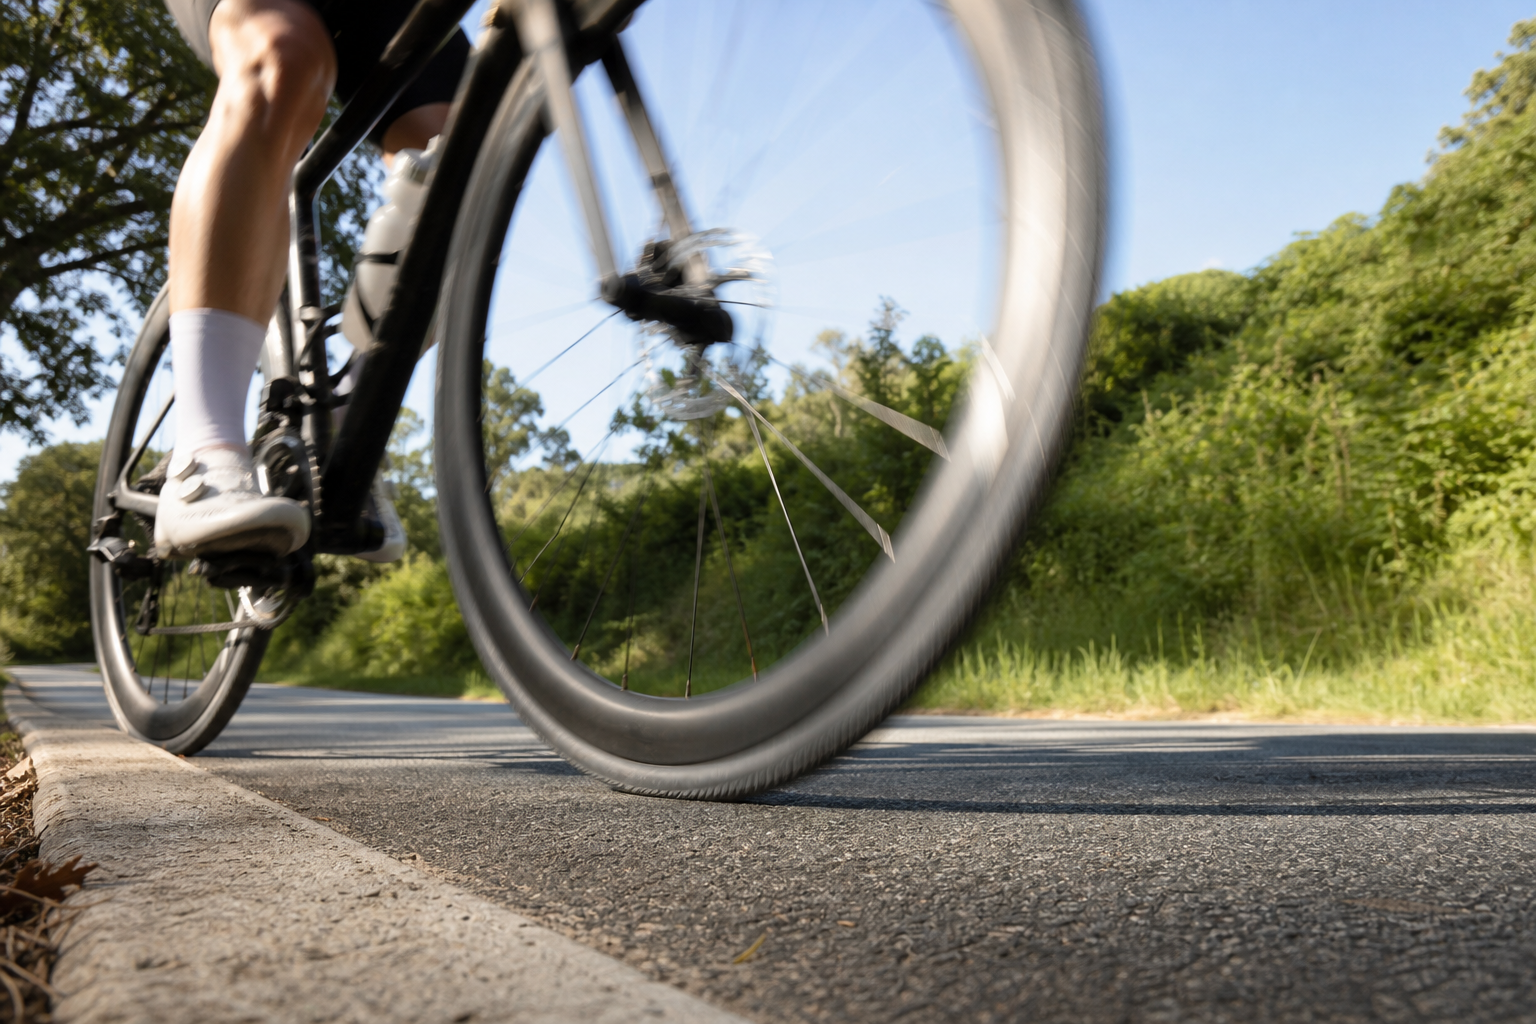
\includegraphics[width=0.58\linewidth]{images/book4/ai/b4-01-bicycle-wheel-blur.png}

{\small A wheel caught by a slow shutter: the spokes near the road, almost at rest, stay sharp; those at the top, moving at twice the bicycle's speed, blur.}
\end{omfigure}


\begin{omfigure}
\begin{tikzpicture}[font=\small, x=1cm, y=1cm, >=Stealth]
  \begin{scope}
    \draw[thick] (-2.6,0) -- (2.6,0);
    \draw[omDef, thick] (0,1.5) circle (1.5);
    \fill (0,1.5) circle (1.5pt) node[below left, font=\footnotesize] {$G$};
    \fill (0,0) circle (1.5pt) node[below, font=\footnotesize] {$I$};
    \draw[omThm, very thick, ->] (0,1.5) -- (1.2,1.5) node[above, font=\footnotesize] {$\vect v_G$};
    \draw[omThm, very thick, ->] (0,3.0) -- (2.4,3.0) node[pos=0.35, above, font=\footnotesize] {$2\vect v_G$};
    \draw[omThm, very thick, ->] (1.5,1.5) -- (2.7,0.3) node[right, font=\footnotesize] {$\sqrt2\,v_G$};
    \draw[omThm, very thick, ->] (-1.5,1.5) -- (-0.3,2.7) node[above left, font=\footnotesize] {$\sqrt2\,v_G$};
    \draw[omThm, thick, ->] (1.06,0.44) -- (1.41,-0.41);
    \draw[omThm, thick, ->] (-1.06,0.44) -- (-0.71,1.29);
    \node[omThm, font=\footnotesize] at (0.3,0.35) {$\vect v_I = \vect 0$};
    \draw[omProp, ->] (-0.5,2.1) arc[start angle=130, end angle=50, radius=0.75] node[midway, above, font=\footnotesize] {$\omega$};
  \end{scope}
  \begin{scope}[xshift=7.6cm]
    \draw[thick] (-2.6,0) -- (2.6,0);
    \draw[omDef, thick] (0,1.5) circle (1.5);
    \fill (0,0) circle (1.5pt) node[below, font=\footnotesize] {$I$};
    \fill (0,1.5) circle (1.5pt);
    \draw[omThm, ->] (0,1.5) -- ($(0,1.5)!0.45!90:(0,0)$);
    \foreach \a in {30,60,...,330} {
      \coordinate (M) at ({1.5*cos(\a)},{1.5+1.5*sin(\a)});
      \draw[omThm, ->] (M) -- ($(M)!0.45!90:(0,0)$);
    }
    \draw[dashed, omExo] (0,0) -- (1.3,2.25);
    \fill (1.3,2.25) circle (1.2pt) node[right, font=\footnotesize] {$M$};
    \node[font=\footnotesize] at (0,-0.8) {$\vect v_M = \vect\Omega\wedge\vect{IM}$};
    \node[font=\footnotesize, align=center] at (0,3.6) {instantaneous rotation\\about the contact point};
  \end{scope}
\end{tikzpicture}

{\small A wheel \omterm{def:b2:rigid-body-mechanics:rolling}{rolling without slipping}. Left: the velocities of a few
points --- zero at the contact point $I$, $v_G = R\omega$ at the centre,
$2v_G$ at the top. Right: every velocity is perpendicular to the segment
joining the point to $I$ and proportional to its length: at each
instant the wheel turns about its contact point.}
\end{omfigure}

\section{Kinetic quantities of a solid}

\begin{proposition}[Momentum, angular momentum, kinetic energy]\label{prop:b2:rigid-body-mechanics:kinetic}
\index{moment of inertia}\index{angular momentum (solid)}\index{kinetic energy (solid)}
For a solid of mass $M$, centre of mass $G$, in a frame $\mathcal R$:
\begin{itemize}
  \item its momentum is $\vect p = M\vect v_G$;
  \item if it rotates about an axis $\Delta$ (fixed in $\mathcal R$, or
        passing through $G$ and fixed in direction) at angular velocity
        $\omega$, its angular momentum \emph{along} that axis is
        $L_\Delta = J_\Delta\,\omega$, where
        \[
        J_\Delta = \sum_i m_i r_i^2 = \int r^2\,\dd m
        \]
        is its \emph{\omterm{prop:b2:rigid-body-mechanics:kinetic}{moment of inertia}} about $\Delta$ ($r$ the distance to
        the axis; unit \unit{kg.m^2});
  \item its kinetic energy is (Koenig) $E_k = \tfrac12Mv_G^2 +
        E_k^*$, where the kinetic energy in the barycentric frame is
        $E_k^* = \tfrac12J_{G}\omega^2$ for a rotation at $\omega$ about
        an axis through $G$ --- and $E_k = \tfrac12J_\Delta\omega^2$ for a
        \omterm{rem:b2:rigid-body-mechanics:motions}{rotation about a fixed axis} $\Delta$.
\end{itemize}
\end{proposition}

\begin{proof}
The momentum and Koenig's theorems were proved in the Year 1 volume for
any system. For the rotation about $\Delta$ through $O$, a point at
distance $r_i$ from the axis has speed $r_i\omega$ on a circle around
the axis; its angular momentum about $O$ projected on $\vect e_\Delta$ is
$m_ir_i^2\omega$ (the other components, which cancel for a symmetric
solid, are not needed here); sum. Kinetic energy: $\sum\tfrac12m_ir_i^2
\omega^2$.
\end{proof}

\begin{remark}[What is admitted]\label{rem:b2:rigid-body-mechanics:tensor}
For an arbitrary rotation $\vect\Omega$ the full vector $\vect L_G$ is
not parallel to $\vect\Omega$ in general: $\vect L_G = \mathbf J\,\vect\Omega$
with $\mathbf J$ the \emph{inertia tensor}, a symmetric matrix whose
eigenvectors are the principal axes. Every solid of this chapter
rotates about a fixed axis or about a symmetry axis through $G$, for
which $\vect L = J\vect\Omega$ exactly; the general case is the Year 3
volume's.
\end{remark}

\begin{proposition}[Moments of inertia]\label{prop:b2:rigid-body-mechanics:inertia}
\index{Huygens' theorem}\index{parallel-axis theorem}
For homogeneous solids of mass $M$, about an axis through $G$: thin rod
of length $\ell$ (axis perpendicular), $J = \tfrac1{12}M\ell^2$; thin hoop
or cylindrical shell of radius $R$ (own axis), $J = MR^2$; disk or full
cylinder, $J = \tfrac12MR^2$; full sphere, $J = \tfrac25MR^2$; spherical
shell, $J = \tfrac23MR^2$. \emph{Huygens' theorem} (parallel axes): about
an axis $\Delta$ parallel to an axis $\Delta_G$ through $G$ at distance
$d$,
\[
J_\Delta = J_{\Delta_G} + Md^2 .
\]
\end{proposition}

\begin{proof}
Rod: $\int_{-\ell/2}^{\ell/2}x^2\,(M/\ell)\dd x = M\ell^2/12$. Disk: rings of
mass $(2M/R^2)r\,\dd r$, $\int_0^R r^2(2M/R^2)r\,\dd r = MR^2/2$. Sphere: by
symmetry $J = \tfrac23\int r^2\dd m$ ($r$ the distance to the centre,
since $x^2 + y^2 = \tfrac23(x^2 + y^2 + z^2)$ on average over the three
axes) and $\int r^2\dd m = \int_0^R r^2(3M/R^3)r^2\dd r = \tfrac35MR^2$.
Huygens: with $\vect r_i$ the vector from $\Delta$ to $m_i$ perpendicular
to the axis and $\vect r_i = \vect d + \vect r_i^*$, $\sum m_ir_i^2 = Md^2
+ 2\vect d\cdot\sum m_i\vect r_i^* + \sum m_ir_i^{*2}$, and the middle sum
vanishes by definition of $G$.
\end{proof}

\begin{example}[A flywheel]\label{ex:b2:rigid-body-mechanics:flywheel}
A steel disk of \qty{50}{kg} and radius \qty{30}{cm}: $J = \tfrac12 \times
50 \times 0.09 = \qty{2.25}{kg.m^2}$; at \qty{3000}{rpm} ($\omega =
\qty{314}{rad/s}$) it stores $\tfrac12J\omega^2 = \qty{111}{kJ}$, the
kinetic energy of a small car at \qty{50}{km/h}. Energy-storage flywheels
spin carbon-fibre rotors at \qty{50000}{rpm} in vacuum on magnetic
\omterm{def:b2:rigid-body-mechanics:pivot}{bearings}: the energy grows as $\omega^2$, the limit is the tensile
strength of the rim.
\end{example}

\section{Dynamics of a solid}

\begin{theorem}[Laws of motion of a solid]\label{thm:b2:rigid-body-mechanics:laws}
\index{angular momentum theorem (solid)}\index{power of forces on a solid}
In a Galilean frame, for a solid subject to external forces $\vect F_i$
applied at points $A_i$:
\begin{enumerate}
  \item (momentum) $M\,\dd\vect v_G/\dd t = \sum\vect F_i$;
  \item (angular momentum about $G$, or about a fixed point $O$)
        $\dd\vect L_G/\dd t = \sum\vect{GA_i}\wedge\vect F_i$; projected on
        a fixed axis $\Delta$ or on an axis through $G$ of fixed
        direction along which the solid rotates at $\omega$:
        $J_\Delta\,\dd\omega/\dd t = \mathcal M_\Delta$, the sum of the
        moments of the external forces about the axis;
  \item (power) the power of a set of forces on a solid is
        $\mathcal P = \vect R\cdot\vect v_A + \vect{\mathcal M}_A\cdot
        \vect\Omega$ for any point $A$ of the solid, with $\vect R$ the
        sum of the forces and $\vect{\mathcal M}_A$ their total moment
        about $A$; \emph{the internal forces of a solid have zero
        power}, and $\dd E_k/\dd t = \mathcal P_{\text{ext}}$.
\end{enumerate}
\end{theorem}

\begin{proof}
(1) and (2) are the theorems of the Year 1 volume for systems of points
(the angular momentum theorem about $G$ holds even when $G$
accelerates, because the inertial forces of the barycentric frame have
zero moment about $G$). (3) With $\vect v_{A_i} = \vect v_A + \vect\Omega
\wedge\vect{AA_i}$: $\sum\vect F_i\cdot\vect v_{A_i} = \vect R\cdot\vect v_A
+ \sum\vect F_i\cdot(\vect\Omega\wedge\vect{AA_i}) = \vect R\cdot\vect v_A +
\vect\Omega\cdot\sum\vect{AA_i}\wedge\vect F_i$ (mixed product). Internal
forces: their sum and their total moment vanish (action--reaction, same
line), hence zero power on a solid --- \emph{not} on a deformable
system. The kinetic energy theorem then keeps only the external power.
\end{proof}

\begin{definition}[Perfect pivot]\label{def:b2:rigid-body-mechanics:pivot}
\index{pivot (perfect)}\index{bearing}
A solid rotates about a fixed axis $\Delta$ in a \emph{perfect pivot}
(an ideal bearing) when the contact forces of the bearing have zero
moment about $\Delta$; they then develop no power ($\vect v_A = \vect 0$
on the axis, $\mathcal M_\Delta = 0$). A real bearing adds a friction
torque $-\Gamma_f\operatorname{sgn}\omega$, or a viscous one $-h\omega$.
\end{definition}

\begin{proposition}[The physical pendulum]\label{prop:b2:rigid-body-mechanics:pendulum}
\index{physical pendulum}\index{compound pendulum}
A solid of mass $M$ swings about a horizontal fixed axis $\Delta$ in a
perfect pivot, its centre of mass at distance $d$ from the axis. With
$\theta$ the angle of $\vect{OG}$ from the downward vertical,
\[
J_\Delta\ddot\theta = -Mgd\sin\theta ,
\]
so that small oscillations have the period $T = 2\pi\sqrt{J_\Delta/Mgd}$
--- that of a simple pendulum of length $\ell_{\text{eq}} = J_\Delta/Md$.
\end{proposition}

\begin{proof}
Angular momentum theorem about $\Delta$: the weight's moment is
$-Mgd\sin\theta$, the pivot's is zero. Linearize.
\end{proof}

\begin{example}[The metre rule]\label{ex:b2:rigid-body-mechanics:rule}
A metre rule pivoted at one end: $J = \tfrac13M\ell^2$ (Huygens from
$\tfrac1{12}M\ell^2$), $d = \ell/2$, $\ell_{\text{eq}} = \tfrac23\ell =
\qty{0.667}{m}$ and $T = \qty{1.64}{s}$ --- a whole-rule pendulum beats
slower than a point mass hung at its centre (\qty{1.42}{s}) and faster
than one at its end (\qty{2.0}{s}).
\end{example}

\begin{omfigure}
\begin{tikzpicture}[font=\small, x=1cm, y=1cm, >=Stealth]
  \begin{scope}
    \fill[pattern=north east lines] (-0.6,3.2) rectangle (0.6,3.45); \draw[thick] (-0.6,3.2) -- (0.6,3.2);
    \fill (0,3.1) circle (2pt) node[left, font=\footnotesize] {$O$};
    \draw[dashed] (0,3.1) -- (0,0.2);
    \draw[omDef, very thick, rotate around={25:(0,3.1)}] (-0.12,3.1) rectangle (0.12,0.3);
    \draw[dashed, omExo] (0,3.1) -- ($(0,3.1)+({2.0*sin(25)},{-2.0*cos(25)})$);
    \coordinate (G) at ({0+1.4*sin(25)},{3.1-1.4*cos(25)});
    \fill[omThm] (G) circle (2pt) node[right, font=\footnotesize] {$G$};
    \draw[omThm, very thick, ->] (G) -- ($(G)+(0,-1.0)$) node[below, font=\footnotesize] {$M\vect g$};
    \draw[<->, omExo] (0,1.5) arc[start angle=-90, end angle=-65, radius=1.6] node[midway, below, font=\footnotesize] {$\theta$};
    \node[font=\footnotesize] at (2.1,2.3) {$J_\Delta\ddot\theta = -Mgd\sin\theta$};
    \draw[<->, omExo] (-0.5,3.1) -- ($(-0.5,3.1)+(0,-1.28)$) node[midway, left, font=\footnotesize] {$d$};
  \end{scope}
  \begin{scope}[xshift=7cm]
    \draw[thick] (-2.5,0) -- (2.5,0);
    \draw[omDef, thick] (0,1.2) circle (1.2);
    \fill (0,1.2) circle (1.5pt);
    \draw[omThm, very thick, ->] (0,1.2) -- (0,-0.3) node[right, font=\footnotesize] {$M\vect g$};
    \draw[omProp, very thick, ->] (0,0) -- (0,1.0) node[left, font=\footnotesize, pos=0.7] {$\vect N$};
    \draw[omExo, very thick, ->] (0,0) -- (-1.0,0) node[below, font=\footnotesize] {$\vect T$};
    \draw[very thick, ->] (0.3,2.6) -- (1.5,2.6) node[right, font=\footnotesize] {$\vect F$};
    \draw[omDef, ->] (-0.5,1.7) arc[start angle=130, end angle=50, radius=0.75] node[midway, above, font=\footnotesize] {$\omega$};
    \node[font=\footnotesize, align=left] at (0,-0.9) {rolling without slipping: $|T| \le fN$};
  \end{scope}
\end{tikzpicture}

{\small Left: the \omterm{prop:b2:rigid-body-mechanics:pendulum}{physical pendulum} --- the weight's moment about the
pivot drives the rotation, the pivot's force has no moment. Right: the
forces on a wheel rolling on a horizontal ground: weight, \omterm{def:b2:rigid-body-mechanics:contact}{normal
reaction} $\vect N$ and tangential friction $\vect T$ at the contact
point, whose magnitude is bounded by Coulomb's law.}
\end{omfigure}

\section{Contact forces and Coulomb friction}

\begin{definition}[Contact force, normal and tangential]\label{def:b2:rigid-body-mechanics:contact}
\index{normal reaction}\index{friction force}
The force exerted by a support on a solid at a contact point $I$ splits
into a \emph{normal reaction} $\vect N$, perpendicular to the common
tangent plane and directed toward the solid ($N \ge 0$: a support can
only push), and a \emph{tangential component} $\vect T$ in the tangent
plane, the \emph{friction force}.
\end{definition}

\begin{theorem}[Coulomb's laws of dry friction]\label{thm:b2:rigid-body-mechanics:coulomb}
\index{Coulomb's laws of friction}\index{coefficient of friction}\index{static friction}\index{kinetic friction}
For two dry solids in contact, with a \emph{\omterm{thm:b2:rigid-body-mechanics:coulomb}{coefficient of friction}} $f$
depending on the materials and their state of surface, but not on the
area of contact nor (to a good approximation) on the speed:
\begin{itemize}
  \item if the solids slip on each other ($\vect v_{\text{slip}} \ne
        \vect 0$), the \omterm{def:b2:rigid-body-mechanics:contact}{friction force} is opposite to the \omterm{def:b2:rigid-body-mechanics:rolling}{slip velocity}
        and of magnitude $\|\vect T\| = f\|\vect N\|$ (\omterm{thm:b2:rigid-body-mechanics:coulomb}{kinetic friction});
  \item if they do not slip, $\|\vect T\| \le f\|\vect N\|$ (\omterm{thm:b2:rigid-body-mechanics:coulomb}{static
        friction}): the \omterm{def:b2:rigid-body-mechanics:contact}{friction force} is then whatever the other laws of
        motion require, within that bound, and its direction is not
        known in advance.
\end{itemize}
A \emph{perfect contact} is the idealization $f = 0$: $\vect T = \vect 0$.
\end{theorem}
\admitted

\begin{remark}[Reading Coulomb's laws]\label{rem:b2:rigid-body-mechanics:reading}
\index{friction cone}
The first law is an equation, the second an inequality --- and that is
the whole difficulty of friction problems. The \emph{method} is to
\emph{assume} no slipping, solve for $\vect T$ and $\vect N$, and
\emph{check} $\|\vect T\| \le f\|\vect N\|$; if the check fails, the
solid slips, $\|\vect T\| = f\|\vect N\|$ opposite to the slip, and the
problem is solved again. Geometrically, the contact force must stay
inside the \emph{\omterm{rem:b2:rigid-body-mechanics:reading}{friction cone}} of half-angle $\varphi$ with $\tan\varphi
= f$. Typical values: rubber on dry asphalt $f \approx 0.8$--$1$, on wet
asphalt $0.4$--$0.6$, on ice $0.1$; steel on steel $0.15$ dry, $0.05$
greased; the static coefficient is in reality slightly larger than the
kinetic one, which is why a skid is hard to stop once started.
\end{remark}

\begin{proposition}[Power of the contact forces; rolling without slipping]\label{prop:b2:rigid-body-mechanics:power}
\index{rolling friction}
The power of the contact forces on a solid moving on a fixed support is
$\mathcal P = \vect T\cdot\vect v_{I\in S}$ (the normal force is
perpendicular to the velocity of the contact point, which is in the
tangent plane). In \emph{\omterm{def:b2:rigid-body-mechanics:rolling}{rolling without slipping}} this power is zero:
friction then does no work, though it may be essential to the motion.
In sliding it is $-f N v_{\text{slip}} < 0$: heat.
\end{proposition}

\begin{proof}
$\mathcal P = (\vect N + \vect T)\cdot\vect v_{I\in S}$ and $\vect
v_{I\in S} = \vect v_{\text{slip}}$ lies in the tangent plane, so only
$\vect T$ contributes; it is zero when the \omterm{def:b2:rigid-body-mechanics:rolling}{slip velocity} is zero, and
$-fNv_{\text{slip}}$ when the solids slip ($\vect T$ opposite to $\vect
v_{\text{slip}}$). Real rolling dissipates a little through the
deformation of tyre and ground (\emph{\omterm{prop:b2:rigid-body-mechanics:power}{rolling friction}}, modelled by a
small torque $\Gamma_r = \mu_rNR$ or an equivalent force $\mu_rN$, with
$\mu_r \approx 0.01$ for a tyre on a road): a different, much smaller
effect.
\end{proof}

\begin{method}[A solid rolling down an incline]\label{met:b2:rigid-body-mechanics:incline}
\index{rolling down an incline}
A homogeneous solid of radius $R$, mass $M$ and \omterm{prop:b2:rigid-body-mechanics:kinetic}{moment of inertia} $J =
kMR^2$ about its axis ($k = 1$ hoop, $\tfrac12$ disk, $\tfrac25$ sphere)
is released on an incline of angle $\alpha$ with friction coefficient
$f$. Assume \omterm{def:b2:rigid-body-mechanics:rolling}{rolling without slipping}:
\begin{enumerate}
  \item momentum along the slope: $M\dot v = Mg\sin\alpha - T$; normal:
        $N = Mg\cos\alpha$;
  \item angular momentum about $G$: $kMR^2\dot\omega = TR$;
  \item no slip: $v = R\omega$, hence $T = kM\dot v$ and
        \[
        \dot v = \frac{g\sin\alpha}{1 + k} , \qquad T = \frac{k}{1 + k}\,
        Mg\sin\alpha ;
        \]
  \item check: $T \le fN \iff \tan\alpha \le f\,\dfrac{1 + k}{k}$.
        Beyond that slope the solid slips, $T = fMg\cos\alpha$, $\dot v =
        g(\sin\alpha - f\cos\alpha)$ and $\dot\omega = fg\cos\alpha/kR$.
\end{enumerate}
Energy check (no slip, friction powerless): $\tfrac12(1 + k)Mv^2 =
Mgh$ gives $v = \sqrt{2gh/(1 + k)}$ --- a sphere beats a disk, which
beats a hoop, independently of mass and radius.
\end{method}

\begin{omfigure}
\begin{tikzpicture}[font=\small, x=1cm, y=1cm, >=Stealth]
  \begin{scope}
    \draw[thick] (0,0) -- (5.5,0) -- (0,2.6) -- cycle;
    \draw (0.9,0) arc[start angle=180, end angle=155, radius=0.9] node[left, font=\footnotesize, xshift=-2pt] {};
    \node[font=\footnotesize] at (4.6,0.25) {$\alpha$};
    \draw (5.5,0) -- (4.7,0) arc[start angle=180, end angle=155, radius=0.8];
    \coordinate (I) at (2.2,1.56);
    \coordinate (G) at ($(I)+(155:-0.0)+(65:0.8)$);
    \draw[omDef, thick] (G) circle (0.8);
    \fill (G) circle (1.5pt);
    \draw[omThm, very thick, ->] (G) -- ($(G)+(0,-1.3)$) node[below, font=\footnotesize] {$M\vect g$};
    \draw[omProp, very thick, ->] (I) -- ($(I)+(65:1.0)$) node[above left, font=\footnotesize, pos=0.9] {$\vect N$};
    \draw[omExo, very thick, ->] (I) -- ($(I)+(155:0.9)$) node[above, font=\footnotesize] {$\vect T$};
    \draw[->, thick] ($(G)+(65:1.1)$) -- ($(G)+(65:1.1)+(-25:1.2)$) node[right, font=\footnotesize] {$\vect v$};
    \node[font=\footnotesize, align=left] at (4.6,1.7) {$\dot v = \dfrac{g\sin\alpha}{1+k}$};
  \end{scope}
  \begin{scope}[xshift=7.6cm]
    \begin{axis}[omaxis, axis x line=bottom, axis y line=left, width=5.6cm, height=4.2cm,
        xlabel={$\alpha$ (deg)}, ylabel={$\dot v/g$}, xmin=0, xmax=90, ymin=0, ymax=1.05,
        xlabel style={at={(axis description cs:0.5,-0.12)}, anchor=north},
        ylabel style={at={(axis description cs:-0.2,0.5)}, rotate=90, anchor=south},
        xtick={0,30,60,90}, ytick={0,0.5,1}, samples=200, legend style={font=\scriptsize, at={(0.03,0.97)}, anchor=north west, draw=none, fill=none}]
      \addplot[omThm, thick, domain=0:56.3] {sin(x)/1.5};
      \addplot[omThm, thick, domain=56.3:90] {sin(x)-0.5*cos(x)};
      \addplot[omDef, thick, dashed, domain=0:90] {sin(x)};
      \legend{disk, , no friction}
      \draw[dotted] (axis cs:56.3,0) -- (axis cs:56.3,0.83);
      \node[font=\scriptsize, anchor=west] at (axis cs:57,0.3) {slips};
    \end{axis}
  \end{scope}
\end{tikzpicture}

{\small Left: forces on a solid \omterm{met:b2:rigid-body-mechanics:incline}{rolling down an incline} --- weight at
$G$, \omterm{def:b2:rigid-body-mechanics:contact}{normal reaction} and friction at the contact point. Right: the
acceleration of a disk ($k = \tfrac12$) as a function of the slope for
$f = 0.5$: it rolls without slipping while $\tan\alpha \le 3f$, then
slips and its acceleration follows $g(\sin\alpha - f\cos\alpha)$, always
below the frictionless $g\sin\alpha$.}
\end{omfigure}

\begin{example}[Why a car needs friction to accelerate]\label{ex:b2:rigid-body-mechanics:car}
A front-wheel-drive car: the engine applies a torque to the front
wheels; the only external horizontal force on the car is the friction
of the road on the tyres, and it is this force that accelerates the
car. With the whole weight on the driven wheels the maximum acceleration
is $fg \approx \qty{8}{m/s^2}$ on dry asphalt --- and half of that if only
half the weight rests on the driven axle; on ice, $\qty{1}{m/s^2}$. The
engine's work is not done by the road (whose contact point is at rest):
it is internal work, converted by the transmission into kinetic energy
--- the same way the internal forces of a walker's muscles, not the
ground, supply the walker's energy.
\end{example}

\begin{example}[The sliding-to-rolling transition]\label{ex:b2:rigid-body-mechanics:bowling}
A bowling ball is released sliding at $v_0$ without spin. \omterm{thm:b2:rigid-body-mechanics:coulomb}{Kinetic
friction} $fMg$ slows the centre ($\dot v = -fg$) and spins the ball up
($\tfrac25MR^2\dot\omega = fMgR$, $\dot\omega = 5fg/2R$) until $v = R\omega$:
at $t_1 = 2v_0/7fg$, with $v_1 = \tfrac57v_0$. From then on it rolls
without slipping at constant speed. Two sevenths of the speed, and
$1 - (\tfrac57)^2\tfrac75 = \tfrac27$ of the kinetic energy, are lost to heat
in the slide --- whatever $f$ is; $f$ only sets how fast.
\end{example}

\begin{omfigure}
\begin{tikzpicture}
\begin{axis}[omaxis, axis x line=bottom, axis y line=left, width=7.6cm, height=4.4cm,
    xlabel={$t/t_1$}, ylabel={}, xmin=0, xmax=2, ymin=0, ymax=1.15,
    xlabel style={at={(axis description cs:0.5,-0.12)}, anchor=north},
    xtick={0,1,2}, ytick={0.714,1}, yticklabels={$\tfrac57v_0$, $v_0$}, samples=100,
    legend style={font=\scriptsize, at={(0.97,0.35)}, anchor=east, draw=none, fill=none}]
  \addplot[omThm, thick, domain=0:1] {1-0.2857*x};
  \addplot[omThm, thick, domain=1:2] {0.714};
  \addplot[omDef, thick, domain=0:1] {0.714*x};
  \addplot[omDef, thick, domain=1:2] {0.714};
  \legend{$v_G$, , $R\omega$}
  \draw[dotted] (axis cs:1,0) -- (axis cs:1,0.714);
\end{axis}
\end{tikzpicture}

{\small A ball released sliding without spin: \omterm{thm:b2:rigid-body-mechanics:coulomb}{kinetic friction} brakes
the centre and spins the ball up, linearly in time, until $R\omega$
catches $v_G$ at $\tfrac57v_0$; from then on the ball rolls without
slipping and friction stops acting.}
\end{omfigure}

\section{Exercises}

\begin{exercise}[$\star$]\label{exo:b2:rigid-body-mechanics:1}
Moments of inertia: (a) a \qty{1.0}{m}, \qty{0.50}{kg} rod about a
perpendicular axis through its centre, then through one end; (b) a
\qty{2.0}{kg} disk of radius \qty{20}{cm} about its axis, then about a
parallel axis through its rim; (c) a \qty{0.16}{kg} billiard ball of
diameter \qty{57}{mm}. (d) A thin hoop and a full disk of the same mass
and radius: which resists spin-up more, and by what factor?
\end{exercise}

\begin{exercise}[$\star$]\label{exo:b2:rigid-body-mechanics:2}
A bicycle rides at \qty{18}{km/h} on wheels of diameter \qty{70}{cm}.
Angular velocity of the wheels; speed, in the ground frame, of the
valve when it is at the top, at the bottom, at the front of the wheel
(height of the axle); speed of the tread relative to the frame of the
bicycle. A stone stuck in the tread comes loose at the top: at what
speed does it leave?
\end{exercise}

\begin{exercise}[$\star$]\label{exo:b2:rigid-body-mechanics:3}
A flywheel is a \qty{40}{kg} steel disk of radius \qty{25}{cm}. (a) Energy
stored at \qty{6000}{rpm}. (b) Constant torque needed to spin it up
from rest in \qty{2.0}{min}; power at the end of the spin-up. (c) In a
bus, it must deliver \qty{20}{kW} for \qty{10}{s}: to what speed does it
slow down? (d) Why are high-speed flywheels run in vacuum?
\end{exercise}

\begin{exercise}[$\star$]\label{exo:b2:rigid-body-mechanics:4}
A uniform disk of radius $R$ swings in a vertical plane about a
horizontal axis through a point of its rim. \omterm{prop:b2:rigid-body-mechanics:kinetic}{Moment of inertia} about
the axis; period of small oscillations for $R = \qty{20}{cm}$; length of
the equivalent simple pendulum. Same questions for the axis at a
distance $R/2$ from the centre. Where should the axis be for the
shortest period?
\end{exercise}

\begin{exercise}[$\star\star$]\label{exo:b2:rigid-body-mechanics:5}
A hoop, a disk and a sphere of the same radius are released together
at the top of a \qty{2.0}{m} high incline of slope \qty{20}{\degree}, $f =
0.30$. (a) Check that all three roll without slipping. (b) Speed at the
bottom for each; order of arrival. (c) Time taken by each. (d) Show that
the \omterm{def:b2:rigid-body-mechanics:contact}{friction force} on the sphere is $\tfrac27Mg\sin\alpha$ and that it does
no work. (e) At what slope would the hoop start to slip? The sphere?
\end{exercise}

\begin{exercise}[$\star\star$]\label{exo:b2:rigid-body-mechanics:6}
\emph{Disk brake.} A wheel and its brake disk have $J = \qty{1.2}{kg.m^2}$
and spin at \qty{900}{rpm}; two pads press on the disk at a mean radius
of \qty{12}{cm}, each with a normal force of \qty{800}{N}, $f = 0.40$.
Braking torque; angular deceleration; time and number of turns to stop;
heat released, and temperature rise of the \qty{1.5}{kg} steel disk
($c = \qty{470}{J/(kg.K)}$) if it keeps it all.
\end{exercise}

\begin{exercise}[$\star\star$]\label{exo:b2:rigid-body-mechanics:7}
\emph{Atwood's machine with a real pulley.} Masses $m_1 = \qty{2.0}{kg}$
and $m_2 = \qty{1.5}{kg}$ hang on a rope over a pulley of radius $R =
\qty{10}{cm}$ and \omterm{prop:b2:rigid-body-mechanics:kinetic}{moment of inertia} $J = \qty{5.0e-3}{kg.m^2}$ on a
perfect pivot; the rope does not slip on the pulley. (a) Why are the two
rope tensions different? (b) Equations for the two masses and the
pulley; acceleration. (c) The two tensions. (d) Compare with the
massless pulley; by energy, recover the acceleration.
\end{exercise}

\begin{exercise}[$\star\star$]\label{exo:b2:rigid-body-mechanics:8}
\emph{The ladder.} A uniform ladder of length $\ell$ and mass $m$ leans
at angle $\theta$ from the horizontal against a smooth vertical wall;
the ground has friction coefficient $f$. (a) Forces and their moments
about the foot; equilibrium equations. (b) Show that equilibrium requires
$\tan\theta \ge 1/2f$. (c) Minimum angle for $f = 0.40$. (d) A person of
mass $3m$ climbs the ladder set at \qty{60}{\degree}: how far up (fraction
of $\ell$) can they go?
\end{exercise}

\begin{exercise}[$\star\star$]\label{exo:b2:rigid-body-mechanics:9}
\emph{Back-spin.} A billiard ball is struck so that it leaves with
centre speed $v_0$ and back-spin $\omega_0$ (rotation opposite to
rolling). Friction coefficient $f$. (a) Equations for $v$ and $\omega$
while sliding. (b) Time at which it starts \omterm{def:b2:rigid-body-mechanics:rolling}{rolling without slipping} and
its speed then, as functions of $v_0$, $R\omega_0$. (c) Condition on
$R\omega_0$ for the ball to come back toward the player. (d) Numbers:
$v_0 = \qty{2.0}{m/s}$, $R\omega_0 = \qty{6.0}{m/s}$, $f = 0.2$,
$R = \qty{2.9}{cm}$.
\end{exercise}

\begin{exercise}[$\star\star\star$]\label{exo:b2:rigid-body-mechanics:10}
\emph{The spool.} A spool (mass $M$, \omterm{prop:b2:rigid-body-mechanics:kinetic}{moment of inertia} $J = kMR^2$ about
its axis, outer radius $R$) rests on a horizontal table; a thread wound
on its inner hub of radius $r < R$ is pulled horizontally with a force
$F$, the thread coming off the \emph{bottom} of the hub. (a) Assuming
\omterm{def:b2:rigid-body-mechanics:rolling}{rolling without slipping}, write the momentum and angular-momentum
equations and find the acceleration of the centre; which way does the
spool roll? (b) \omterm{def:b2:rigid-body-mechanics:contact}{Friction force} required, and the condition on $F$ for
no slipping. (c) Same questions if the thread is pulled at an angle
$\beta$ above the horizontal; show that the spool stays still when
$\cos\beta = r/R$, and explain geometrically (instantaneous axis through
the contact point). (d) What happens for $\cos\beta < r/R$?
\end{exercise}

\begin{exercise}[$\star\star\star$]\label{exo:b2:rigid-body-mechanics:11}
\emph{Where to hit a billiard ball.} A cue delivers a horizontal
impulse $P$ (very short force) to a ball of radius $R$ at rest, at
height $h$ above the table. (a) Momentum and angular momentum just after
the hit (friction negligible during the hit). (b) Show that the ball
rolls without slipping at once if $h = \tfrac75R$, has top-spin above,
back-spin below. (c) For $h = R$ (centre hit), how far does the ball
slide before rolling, with $f = 0.2$ and $v_0 = \qty{3}{m/s}$? (d) Why is
the cushion of a billiard table built at height $\tfrac75R$?
\end{exercise}

\begin{exercise}[$\star\star\star$]\label{exo:b2:rigid-body-mechanics:12}
\emph{Cylinder in a bowl.} A full cylinder of radius $r$ rolls without
slipping inside a fixed cylindrical surface of radius $R > r$, axes
horizontal and parallel. Let $\theta$ be the angle of the line of
centres from the vertical. (a) Express the angular velocity of the
cylinder about its own axis in terms of $\dot\theta$ (hint: the contact
point is at rest). (b) Kinetic energy and potential energy; show the
period of small oscillations is $T = 2\pi\sqrt{3(R - r)/2g}$. (c) Compare
with a point sliding without friction in the bowl. (d) Minimum friction
coefficient for \omterm{def:b2:rigid-body-mechanics:rolling}{rolling without slipping} at amplitude $\theta_0$
(small angles).
\end{exercise}

\section{Problem: A vehicle on wheels}

\begin{problem}[{Weekend problem --- what a car asks of its tyres:
rolling, accelerating, braking, and the one force that does it all}]
\label{pb:b2:rigid-body-mechanics:1}

A car of mass $M = \qty{1200}{kg}$ has a wheelbase $L = \qty{2.6}{m}$; its
centre of mass is at height $h = \qty{0.55}{m}$ and at horizontal distances
$a = \qty{1.1}{m}$ from the front axle and $b = \qty{1.5}{m}$ from the rear
axle. Each of the four wheels has radius $R = \qty{0.31}{m}$, mass $m =
\qty{15}{kg}$ and \omterm{prop:b2:rigid-body-mechanics:kinetic}{moment of inertia} $J = \qty{1.0}{kg.m^2}$ about its axle.
Tyre--road friction coefficient $f = 0.80$ (dry); rolling-friction
coefficient $\mu_r = 0.012$. $g = \qty{9.81}{m/s^2}$.

\medskip
\noindent\textbf{Part I --- Rolling.}
\begin{enumerate}
  \item The car drives at $v = \qty{90}{km/h}$. Angular velocity of the
        wheels; velocity, in the road frame, of the top, bottom and
        front points of a tyre.
  \item Total kinetic energy of the car, separating the translation of
        the whole and the rotation of the four wheels; what fraction do
        the wheels' rotations represent?
  \item At rest on level ground, normal forces $N_f$ (both front wheels
        together) and $N_r$ (both rear) by the momentum and
        angular-momentum equations --- which axle carries more?
  \item The rolling-friction torque on each wheel is $\mu_rNR$. Power
        dissipated by \omterm{prop:b2:rigid-body-mechanics:power}{rolling friction} at \qty{90}{km/h}; compare with
        the aerodynamic drag $\tfrac12\rho C_xSv^2$ with $C_xS =
        \qty{0.70}{m^2}$, $\rho = \qty{1.2}{kg/m^3}$.
  \item The engine is cut and the car coasts on level ground: write the
        equation for $v(t)$ (include the wheels' inertia as an effective
        mass) and estimate the distance to slow from \qty{90}{km/h} to
        \qty{45}{km/h}, neglecting drag; then including only drag.
\end{enumerate}

\medskip
\noindent\textbf{Part II --- Accelerating.}
The car is front-wheel drive; the engine applies a torque $\Gamma$ to
the two front wheels together. Neglect drag and \omterm{prop:b2:rigid-body-mechanics:power}{rolling friction} here.
\begin{enumerate}[resume]
  \item Draw the external forces on the whole car. Which force
        accelerates it? What is the power of the road on the car, and
        where does the kinetic energy come from?
  \item Write the momentum equation of the car, the angular-momentum
        equation of the front wheels about their axle, and the
        no-slip condition; show that the acceleration is $\dot v =
        \Gamma/R\,/\,(M + 4J/R^2)$ and compute the effective mass.
  \item Angular momentum about the centre of mass for the whole car
        (treat the wheels' angular momenta as negligible): show that
        the load transfer under acceleration $\dot v$ is $N_r - N_r^0 =
        Mh\dot v/L$ --- the front axle is unloaded, the rear loaded.
  \item Maximum acceleration without the driven (front) wheels
        spinning: show that $\dot v_{\max} = fgb/(L + fh)$ and compute
        it; the same for a rear-wheel-drive car, $\dot v_{\max} =
        fga/(L - fh)$. Which layout accelerates harder, and why do
        dragsters put the weight at the back?
  \item Engine torque at the wheels needed for $\dot v_{\max}$; the
        corresponding power at \qty{50}{km/h}.
  \item The same car on ice ($f = 0.10$): maximum acceleration and the
        time to reach \qty{50}{km/h}.
  \item What does the \omterm{def:b2:rigid-body-mechanics:contact}{friction force} on the front tyres do to the tyre
        --- sliding or not --- and why does a spinning wheel on ice
        accelerate the car \emph{less} than a gripping one?
\end{enumerate}

\medskip
\noindent\textbf{Part III --- Braking.}
\begin{enumerate}[resume]
  \item The brakes apply a torque to each wheel. Show that, for a wheel
        that keeps rolling, the braking force on the car is the
        road's friction on the tyre, and that the brake torque is
        limited by $fN_iR$ per wheel.
  \item Load transfer under deceleration $\gamma$: front axle load
        $N_f = Mg\,b/L + Mh\gamma/L$; numbers at $\gamma = fg$.
  \item Maximum deceleration with all four wheels at the limit of
        slipping; stopping distance from \qty{90}{km/h} on dry road, and
        on wet road ($f = 0.45$).
  \item If the brakes are set so that front and rear torques are equal,
        which axle locks first at hard braking? Why is a locked rear
        axle dangerous (think of the direction of the \omterm{def:b2:rigid-body-mechanics:contact}{friction force}
        on a sliding tyre)?
  \item A wheel locks and slides: deceleration from the road, and what
        fraction of the peak braking is lost with $f_{\text{kinetic}} =
        0.7$ vs $f_{\text{static}} = 0.8$. Explain what an anti-lock
        system does and why it pulses the brakes.
  \item Heat released in the brakes from \qty{90}{km/h}; temperature
        rise of four \qty{6}{kg} steel disks ($c = \qty{470}{J/(kg.K)}$);
        why do mountain roads have runaway-truck ramps?
  \item An electric car recovers braking energy through its motor at
        \qty{70}{\%} efficiency: energy recovered per stop from
        \qty{90}{km/h}; number of such stops a \qty{50}{kWh} battery is
        worth.
\end{enumerate}

\medskip
\noindent\textbf{Part IV --- Cornering and a wheel off the ground.}
\begin{enumerate}[resume]
  \item The car turns on a flat road on a circle of radius
        $\rho = \qty{50}{m}$ at $v$: the \omterm{def:b2:rigid-body-mechanics:contact}{friction forces} must supply
        $Mv^2/\rho$. Maximum cornering speed on dry and on wet road.
  \item Angular-momentum about the centre of mass along the direction of
        motion: show that the outer wheels are loaded by $\Delta N =
        Mv^2h/\rho w$ where $w = \qty{1.5}{m}$ is the track; speed at
        which the inner wheels lift ($\Delta N = Mg/2$), and compare
        with the skidding speed: does this car roll over or skid first?
  \item The bend is banked at an angle $\beta$. Show that at the speed
        $v = \sqrt{g\rho\tan\beta}$ no friction is needed at all; value
        for $\beta = \qty{10}{\degree}$.
  \item A wheel is jacked off the ground and spun by hand to
        \qty{60}{rpm}; its \omterm{def:b2:rigid-body-mechanics:pivot}{bearing} exerts a friction torque of
        \qty{0.05}{N.m}. How long does it spin? Kinetic energy lost.
  \item The spinning wheel is dropped onto the road (car at rest, wheel
        at \qty{60}{rpm}, $N = \qty{3}{kN}$): sliding time before it stops,
        and the distance the car would be pushed if it were free to
        roll (treat the car as a mass $M$ on free wheels, neglect the
        other wheels' inertia).
  \item Sum up in one table: the four regimes (rolling, accelerating,
        braking, cornering), the force that acts in each and the
        Coulomb bound it must respect.
\end{enumerate}
\end{problem}
